% Paquets généraux
\documentclass[a4paper,12pt,titlepage]{article}
\usepackage[T1]{fontenc}
\usepackage[utf8]{inputenc}
\usepackage[french]{babel}
\usepackage[gen]{eurosym}
%\usepackage[dvips]{graphicx}
\usepackage{fancyhdr}
\usepackage{pdfpages} 
\usepackage{multido}
\usepackage{moreverb}
\usepackage{hyperref}
%\usepackage{textcomp}
\usepackage{verbatim}
\usepackage{moreverb}
\usepackage{listings}
\usepackage{minted}
\usepackage{eso-pic}
\usepackage{enumitem}
\usepackage{comment}
\usepackage{boxedminipage}
\usepackage[french,onelanguage, boxruled,linesnumbered]{algorithm2e}


\newcommand{\auteurun}{Juliette Genzmer}
\newcommand{\auteurdeux}{Willie Robert}
\newcommand{\auteurtrois}{Renaud Costadoat}
\newcommand{\institute}{Lycée Dorian}
\newtheorem{solution}{Solution}


\newcommand{\nom}{Porte conteneur}
\newcommand{\sequence}{03}
\newcommand{\num}{04}
\newcommand{\type}{TD}
\newcommand{\descrip}{Résolution d'un problème en utilisant des méthodes algorithmiques}
\newcommand{\competences}{Alt-C3: Concevoir un algorithme répondant à un problème précisément posé}

\usepackage{color}
\usepackage{xcolor}
\usepackage{colortbl}
\usepackage{helvet}
\renewcommand{\familydefault}{\sfdefault}
\usepackage{amsfonts}
\usepackage{amsmath}
%\usepackage{xspace}
\usepackage{varioref}
\usepackage{tabularx}
%\usepackage{floatflt}
\usepackage{graphics}
\usepackage{wrapfig}
\usepackage{textcomp}
\usepackage{tikz}
\usepackage{wrapfig}
\usepackage{gensymb}
\usepackage{ifthen}
\usepackage{cancel}
\usepackage{etoolbox}
\usepackage{multirow}
%\usepackage{boxedminipage}
\definecolor{gris25}{gray}{0.75}
\definecolor{bleu}{RGB}{18,33,98}
\definecolor{bleuf}{RGB}{42,94,171}
\definecolor{bleuc}{RGB}{231,239,247}
\definecolor{rougef}{RGB}{185,18,27}
\definecolor{rougec}{RGB}{255,188,204}%255,230,231
\definecolor{vertf}{RGB}{103,126,82}
\definecolor{vertc}{RGB}{220,255,191}
\definecolor{forestgreen}{rgb}{0.13,0.54,0.13}
\definecolor{blcr}{rgb}{0.59,0.69,0.84}
\definecolor{blfr}{rgb}{0.32,0.51,0.75}
\definecolor{orfr}{rgb}{0.90,0.42,0.15}
\definecolor{orcr}{rgb}{0.90,0.65,0.50}
\definecolor{orangef}{rgb}{0.659,0.269,0.072}
\definecolor{orange}{rgb}{0.58,0.35,0.063}
\definecolor{orangec}{rgb}{0.43,0.32,0.25}
\definecolor{rcorrect}{rgb}{0.6,0,0}
\definecolor{sequence}{rgb}{0.75,0.75,0.75}
\definecolor{competences}{rgb}{0.61,0.73,0.35}
\definecolor{grisf}{HTML}{222222}
\definecolor{grisc}{HTML}{636363}
\definecolor{normal}{HTML}{4087c4}
\definecolor{info}{HTML}{5bc0de}
\definecolor{success}{RGB}{92,184,92}
\definecolor{warning}{RGB}{240,173,78}
\definecolor{danger}{RGB}{217,83,79}
\hypersetup{                    % parametrage des hyperliens
    colorlinks=true,                % colorise les liens
    breaklinks=true,                % permet les retours à la ligne pour les liens trop longs
    urlcolor= blfr,                 % couleur des hyperliens
    linkcolor= orange,                % couleur des liens internes aux documents (index, figures, tableaux, equations,...)
    citecolor= forestgreen                % couleur des liens vers les references bibliographiques
    }

% Mise en page
\pagestyle{fancy}

\setlength{\hoffset}{-18pt}

\setlength{\oddsidemargin}{0pt} 	% Marge gauche sur pages impaires
\setlength{\evensidemargin}{0pt} 	% Marge gauche sur pages paires
\setlength{\marginparwidth}{00pt} 	% Largeur de note dans la marge
\setlength{\headwidth}{481pt} 	 	% Largeur de la zone de tête (17cm)
\setlength{\textwidth}{481pt} 	 	% Largeur de la zone de texte (17cm)
\setlength{\voffset}{-18pt} 		% Bon pour DOS
\setlength{\marginparsep}{7pt}	 	% Séparation de la marge
\setlength{\topmargin}{-30pt} 		% Pas de marge en haut
\setlength{\headheight}{55pt} 		% Haut de page
\setlength{\headsep}{20pt} 		% Entre le haut de page et le texte
\setlength{\footskip}{30pt} 		% Bas de page + séparation
\setlength{\textheight}{700pt} 		% Hauteur de l'icone zone de texte (25cm)
\setlength\fboxrule{1 pt}
\renewcommand{\baselinestretch}{1}
\setcounter{tocdepth}{1}
\newcommand{\cadre}[2]
{\fbox{
  \begin{minipage}{#1\linewidth}
   \begin{center}
    #2\\
   \end{center}
  \end{minipage}
 }
}

\newcounter{num_quest} \setcounter{num_quest}{0}
\newcounter{num_rep} \setcounter{num_rep}{0}
\newcounter{num_cor} \setcounter{num_cor}{0}

\newcommand{\question}[1]{\refstepcounter{num_quest}\par
~\ \\ \parbox[t][][t]{0.15\linewidth}{\textbf{Question \arabic{num_quest}}}\parbox[t][][t]{0.85\linewidth}{#1\label{q\the\value{num_quest}}}\par\par
}



\newcommand{\reponse}[0]{\refstepcounter{num_rep}\par
~\ \\ \parbox[t][][t]{0.15\linewidth}{\textbf{Question \arabic{num_rep}}}}

\newcommand{\cor}
{\refstepcounter{num_cor}
\noindent
\rule{\linewidth}{.5pt}
\textbf{Question \arabic{num_cor}:} \\
}



% En tête et pied de page
\lhead{\nom}
\rhead{
\includegraphics[width=2cm]{../../../img/logo}}
\lfoot{David Aubert, Renaud Costadoat}
\rfoot{Page \thepage}
\cfoot{}

\newlength{\RoundedBoxWidth}
\newsavebox{\GrayRoundedBox}
\newenvironment{GrayBox}[1][\dimexpr\textwidth-4.5ex]%
   {\setlength{\RoundedBoxWidth}{\dimexpr#1}
    \begin{lrbox}{\GrayRoundedBox}
       \begin{minipage}{\RoundedBoxWidth}}%
   {   \end{minipage}
    \end{lrbox}
    \begin{center}
    \begin{tikzpicture}%
       \draw node[draw=bleuf,fill=bleuc,rounded corners,%
             inner sep=2ex,text width=\RoundedBoxWidth]%
             {\usebox{\GrayRoundedBox}};
    \end{tikzpicture}
    \end{center}}

\fancypagestyle{correction}{%
  \fancyhf{}
  \lhead{\colorbox{danger}{\begin{minipage}{0.65\paperwidth} \textcolor{white}{\textbf{Correction}} \end{minipage}} }
  \rhead{
\includegraphics[width=2cm]{../../../img/logo}}
  \lfoot{Juliette Genzmer, Willie Robert, Renaud Costadoat}
  \rfoot{\colorbox{danger}{\begin{minipage}{0.3\paperwidth} \begin{flushright}\textcolor{white}{\textbf{Correction}}\end{flushright} \end{minipage}} }}

\renewcommand{\footrulewidth}{0.4pt}


\newcommand{\BackgroundPic}{%
\put(0,0){%
\parbox[b][\paperheight]{\paperwidth}{%
\vfill
\begin{center}
\hspace{0.5cm}\vspace{0.5cm}

\includegraphics[width=\paperwidth,height=\paperheight,%
keepaspectratio]{../../../img/fond5}%
\end{center}
\vfill
}}}

\newcommand{\goforum}{
\begin{figure}[ht!]
\begin{center}
 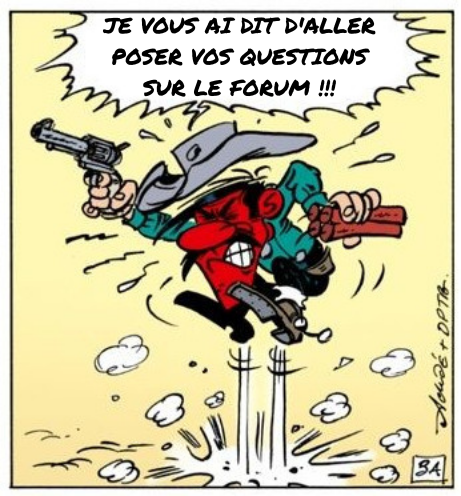
\includegraphics[width=0.7\linewidth]{../../../img/go_forum}
\end{center}
\label{go_forum}
\caption{J'pète les plombs}
\end{figure}}

\newcommand{\BackgroundPicdeux}{%
\put(25,-30){%
\parbox[b][\paperheight]{\paperwidth}{%
\vfill
\begin{center}

\includegraphics[width=\paperwidth,height=\paperheight,%
keepaspectratio]{../../../img/fond6}%
\end{center}
\vfill
}}}

\setenumerate[1]{align=left,label=\arabic*}
\setenumerate[2]{before=\stepcounter{enumi},label*=.\arabic*,leftmargin=1.2em,align=left}

\begin{document}


\pagestyle{fancy}

\AddToShipoutPicture{\BackgroundPicdeux}

\begin{center}
{\Large\bf {\type} \no {\numero} -- \descrip}
\end{center}

\SetKw{KwFrom}{de} 

\begin{boxedminipage}{.9\textwidth} 
\begin{itemize}
 \item Faire tous les exercices dans un fichier {NomPrenom.py} à sauvegarder,
 \item mettre en commentaire l'exercice et la question traités (ex: \# Exercice 1),
 \item ne pas oublier pas de commenter ce qui est fait dans votre code (ex: \# Je crée une fonction pour calculer la racine d'un nombre),
 \item compte tenu du fait que l'épreuve est à distance, il n'est pas possible de demander un déblocage pour une question,
 \item il faut vérifier avant de déposer le fichier (sur \href{https://www.ptsi-dorian.net/depot-de-fichiers}{https://www.ptsi-dorian.net/depot-de-fichiers}), que le code peut s'exécuter et qu'il affiche les résultats que vous attendez.
\end{itemize}
\end{boxedminipage}

~\

Les documents ressources pour ce sujet sont disponibles à l'adresse suivante: \\
\href{https://github.com/Costadoat/Informatique/raw/master/DS/2023-2024/DS04/ressources.zip}{https://github.com/Costadoat/Informatique/raw/master/DS/2023-2024/DS04/ressources.zip}

Vous devez extraire les fichiers du .zip ou les télécharger 1 par 1 depuis le dossier github.

\vspace{-0.5cm}

\section{La maquette de la Licorne}

Dans une de ses aventures, Tintin doit rechercher \og Le trésor de Rackham le Rouge\fg. Nous allons, avec cette épreuve, l'aider dans cette recherche.

Dans le livre précédent \og Le secret de la Licorne \fg, Tintin achète une maquette de bateau sur un marché.

\begin{figure}[ht!]
\begin{center}
 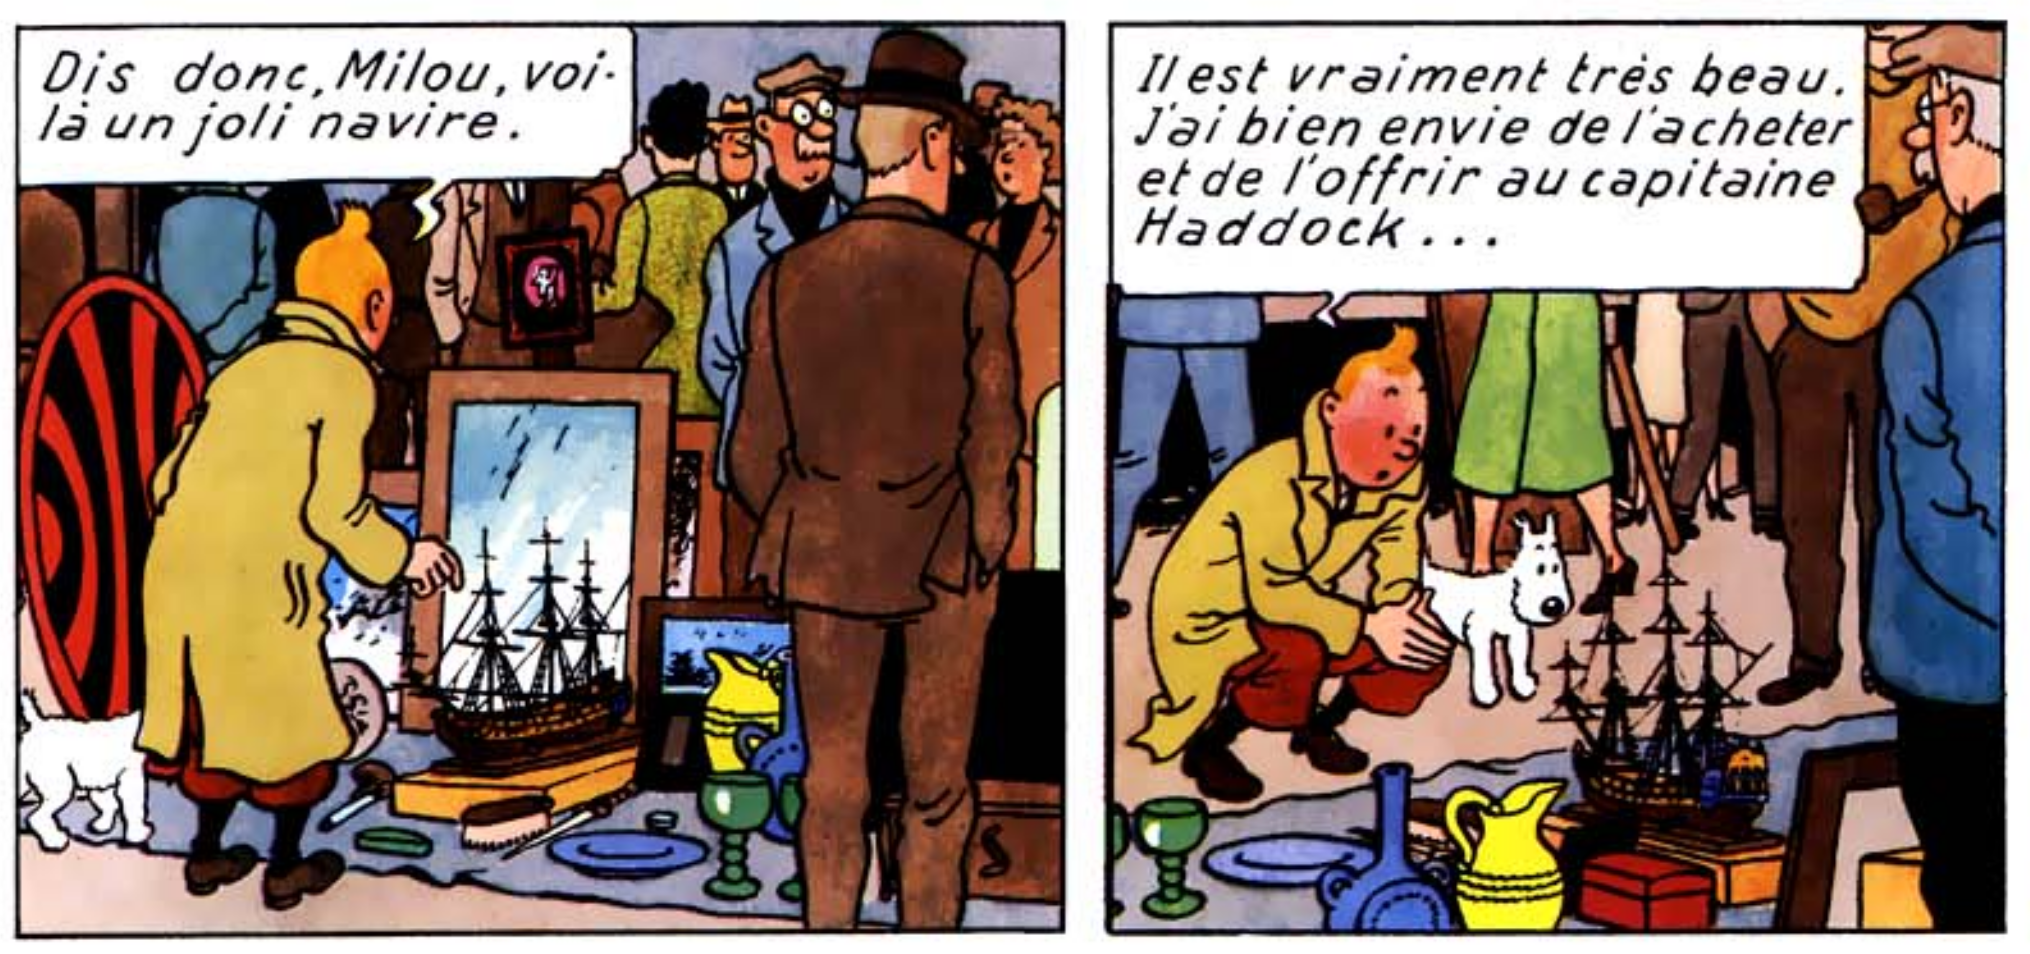
\includegraphics[width=.7\textwidth]{img/marche}
\end{center}
\vspace{-0.8cm}
\caption{\label{fig01} Tintin achète une maquette de la Licorne au marché}
\end{figure}

\begin{wrapfigure}[9]{r}{0.3\textwidth}
\vspace{-\baselineskip}
    \centering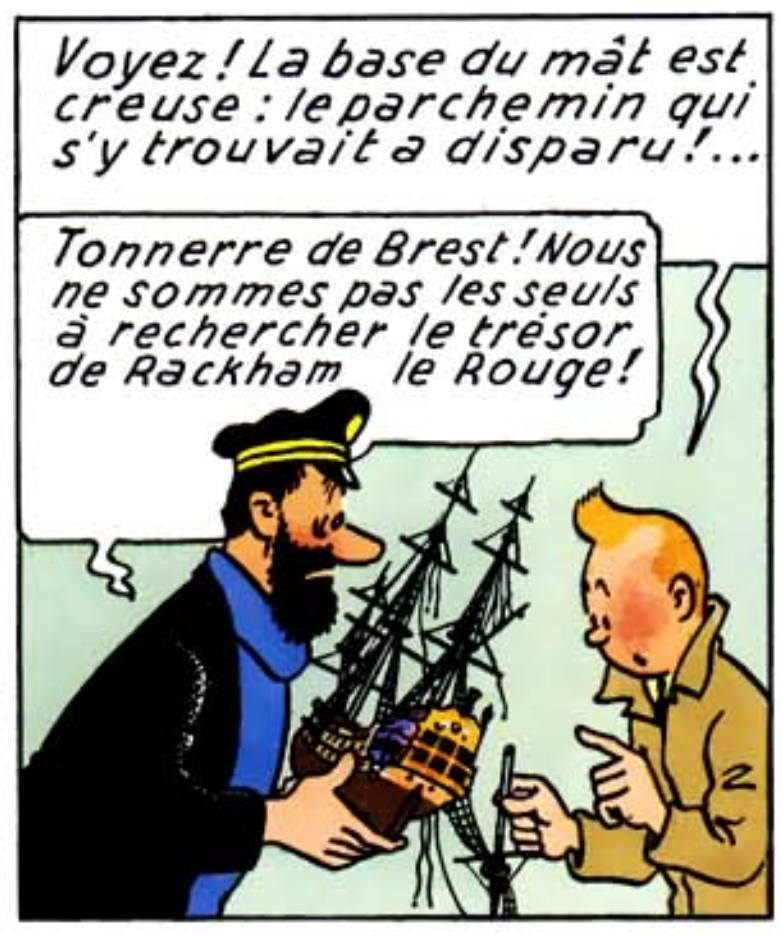
\includegraphics[width=0.75\linewidth]{img/decouverte}
	\caption{\label{fig02} Découverte du parchemin}
\end{wrapfigure}

Il s'agit d'une maquette de la Licorne, un bateau ayant appartenu au chevalier de Hadoque, un ancêtre du Capitaine Haddock, et il en existe 3 parfaitement identiques.

Après quelques péripéties, il découvre qu'un parchemin se cachait à l'intérieur du mat creux des trois maquettes.

Ces parchemins correspondent aux fichiers \verb?parchemin1.png?, \verb?parchemin2.png? et \verb?parchemin3.png?.

Les images sont codées en RGBA, avec \textbf{des valeurs allant de 0 à 1}.


\newpage

\question{A l'aide de la bibliothèque \verb?matplotlib.image? et \verb?matplotlib.pyplot?, \textbf{ouvrir} \verb?parchemin1.png?, \verb?parchemin2.png? et \verb?parchemin3.png? et les stocker dans 3 variables (\verb?parchemin1?, \verb?parchemin2? et \verb?parchemin3?). \textbf{Afficher} seulement \verb?parchemin1.png? à l'aide d'une commande \verb?imshow?.}

~\

Les parchemins font apparaître un message codé quand on les superpose.

Pour cela, nous allons additionner \verb?parchemin1?, \verb?parchemin2? et \verb?parchemin3? et afficher l'image qui en résulte.

Il y a pourtant un problème avec cette addition. Pour certains pixels, la valeur dépasse 1 (on rappelle que 1 est la valeur maximale).

\question{\textbf{Créer} la variable \verb?parchemin? obtenue en faisant la somme des 3 variables définies à la question \ref{q1}. Parcourir chaque pixel de l'image afin de \textbf{saturer} les valeurs à 1. Ex: si la valeur RGBA du pixel i,j a pour valeur [1.2,0.6,0,1], on la remplace par [1,0.6,0,1].}

~\

Il existe plusieurs méthodes pour effectuer cette opération, elles sont toutes acceptées.

Le message secret apparaît et il indique les coordonnées de l'épave de la licorne qui est sensée contenir le trésor.

\section{Recherche de l'épave du bateau}

La suite va tenter de déterminer où se trouve l'épave à partir de ces coordonnées. Si vous n'avez pas réussi la première partie, vous pouvez essayer de reconstituer les coordonnées à partir des 3 parchemins.

Les coordonnées présentes sur le message sont de la forme:
\begin{center}
AA°BB'CC"W DD°EE'FF"N
\end{center}

Ces coordonnées DMS, se lisent comme suit : AA degrés, BB minutes (60ème de degré), CC secondes (60ème de minute) vers l'ouest (W) à partir du méridien origine. DD degrés, EE minutes (60ème de degré), FF secondes (60ème de minute) vers le nord (N) à partir de l'équateur. Où AA, BB, CC, DD, EE, FF sont des entiers.

Il est alors possible de convertir ces coordonnées en coordonnées DD qui ne contiennent que les valeurs en degré mais sous forme de float signés. Cela reviendrait, pour l'expression du temps, à convertir 12h30min en 12.5h. Le signe vient du sens de déplacement, \og + \fg si le déplacement est vers le Nord ou vers l'Est et \og - \fg si le déplacement est vers le Sud ou vers l'Ouest. 

\question{\textbf{Proposer} une fonction \verb?dmstodd(coord,dir)? qui retourne un float au format DD à partir des coordonnées DMS. \textbf{Montrer} que \verb?dmstodd([20,37,42],'N')? retourne \verb?20.628333333333334?.}

\newpage

Après de longues fouilles, les explorateurs se rendent compte que l'épave ne se trouve pas à l'endroit prévu. Alors qu'ils s'apprêtent à rentrer bredouilles, Tintin a une idée.

\begin{figure}[ht!]
\begin{center}
 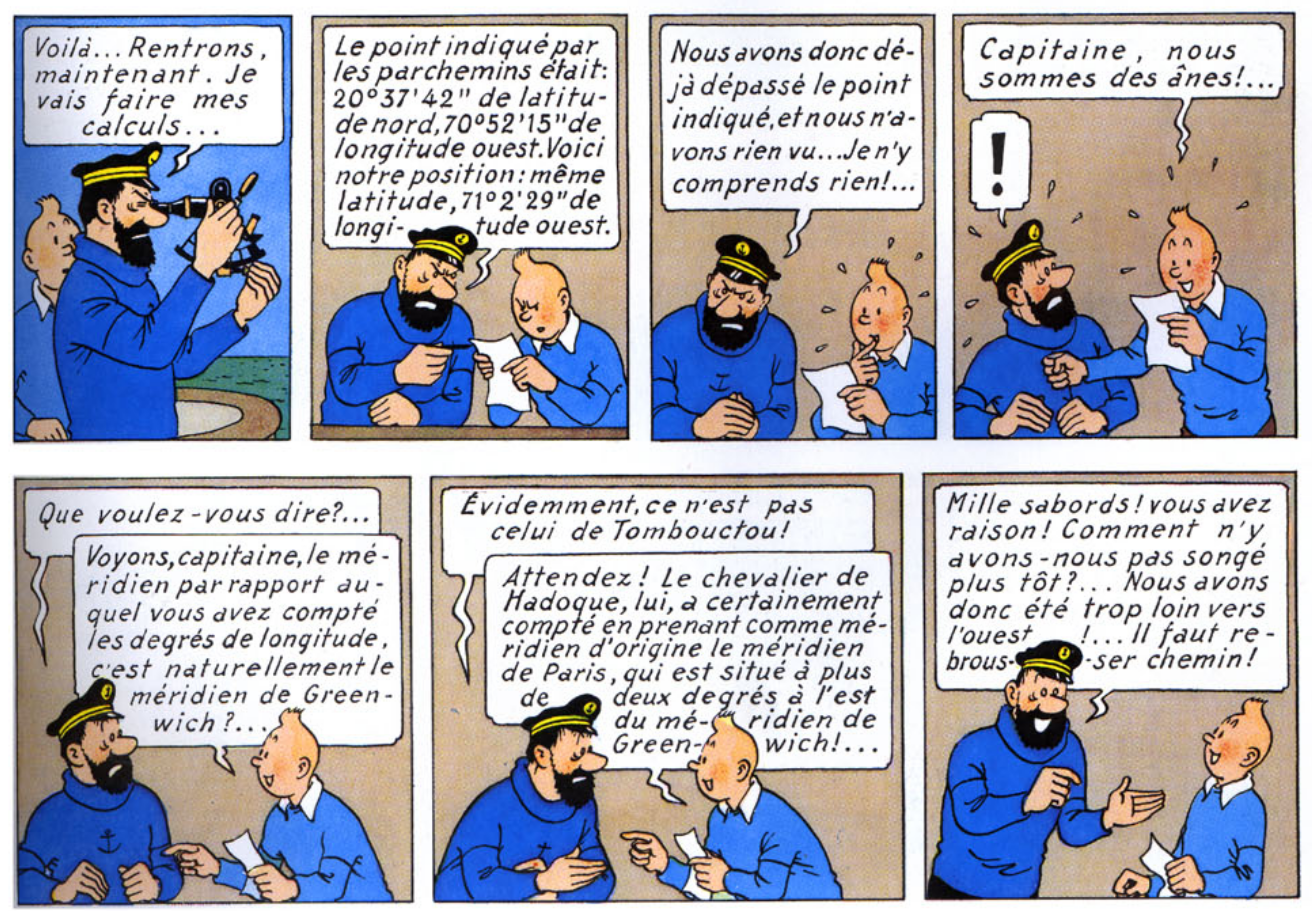
\includegraphics[width=.8\textwidth]{img/erreur_coordonnees}
\end{center}
\vspace{-0.8cm}
\caption{\label{fig03} Tintin comprend qu'ils se sont trompés dans le calcul des coordonnées}
\end{figure}

En effet, du temps du chevalier de Haddock, le méridien d'origine n'était pas celui de Greenwich (près de Londres) mais celui de Paris, situé 2°20'13" à l'est de celui de Greenwich.

\question{\textbf{Proposer} les nouvelles coordonnées de l'épave au format DD et \textbf{déterminer} quelle distance doit parcourir le bateau afin de regagner l'emplacement réel de l'épave.}

~\

On donne la fonction distance qui retourne la distance en km entre deux points A et B désignés par leurs coordonnées (Lattitude, Longitude) exprimées au format DD:

\begin{minted}{python}
def distance(pointA,pointB):
    rayon_terre=6361
    phi1=pointA[0]*np.pi/180
    phi2=pointB[0]*np.pi/180
    deltalambda=(pointB[1]-pointA[1])*np.pi/180
    return np.arccos(np.sin(phi1)*np.sin(phi2) \
    +np.cos(phi1)*np.cos(phi2)*np.cos(deltalambda))*rayon_terre
\end{minted}


L'épave était bien là, mais malgré des explorations poussées, ils ne trouvent aucun trésor. Ils trouvent par contre des documents signifiant que le chevalier de Hadoque était propriétaire du Château de Moulinsard. Or celui-ci est à vendre et Tintin et le capitaine Haddock décident de visiter ses caves.

\begin{figure}[ht!]
\begin{center}
 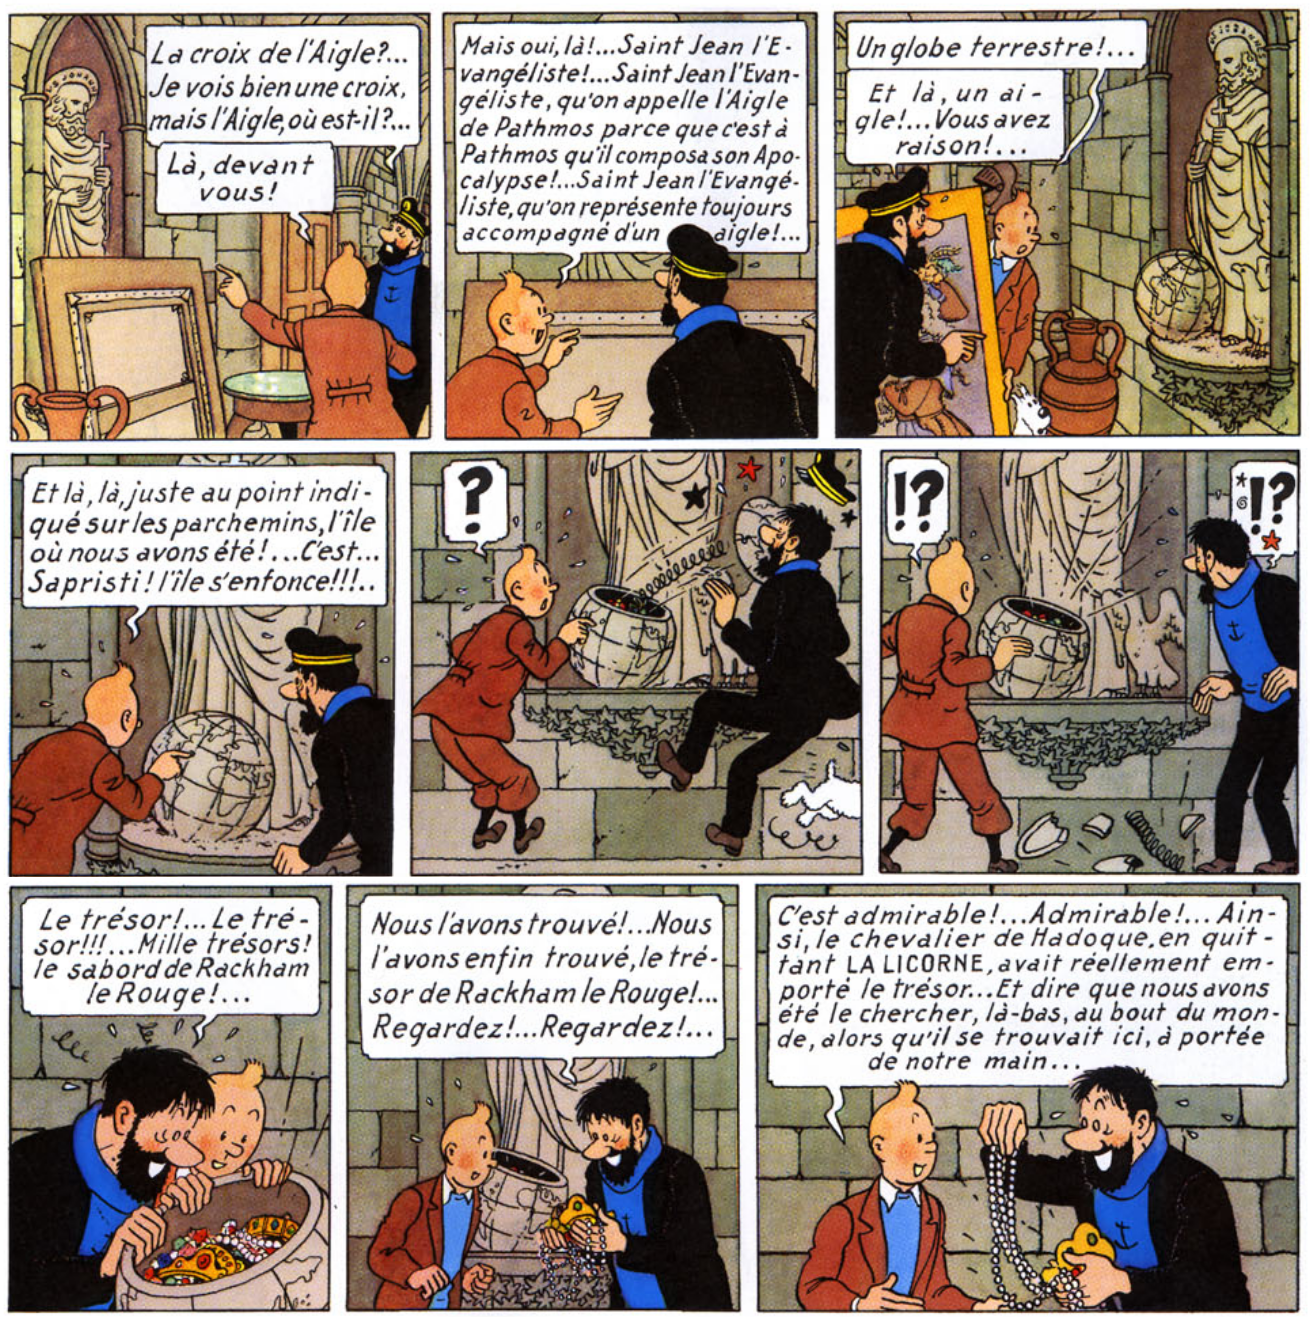
\includegraphics[width=.8\textwidth]{img/decouverte_tresor}
\end{center}
\vspace{-0.8cm}
\caption{\label{fig04} Tintin et la capitaine trouvent le trésor au château de Moulinsard}
\end{figure}

Passons à la suite pour découvrir ce que contenait ce trésor.

\section{Le trésor de Rackham le Rouge}

\begin{wrapfigure}[10]{r}{0.4\textwidth}
\vspace{-\baselineskip}
    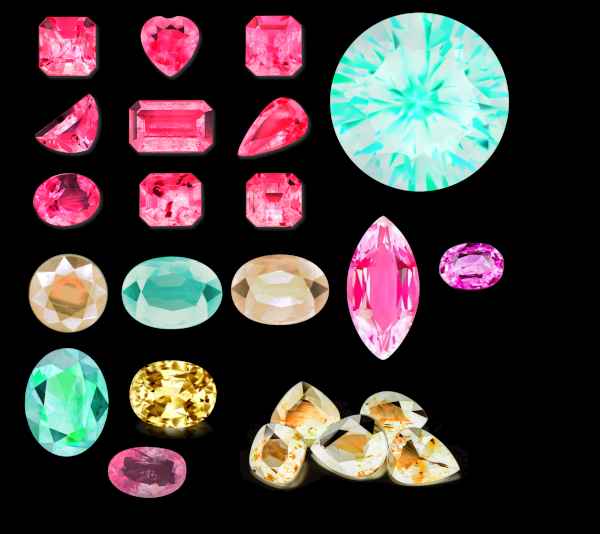
\includegraphics[width=0.85\linewidth]{tresor}
    \caption{\label{fig05} Négatif photo du trésor}
\end{wrapfigure}

Le trésor est magnifique, il contient des rubis (rouges), des saphirs (bleus) et des émeraudes (vertes). L'image \verb?tresor.png? présente dans le dossier de travail contient une photo en négatif (couleurs inversées) d'une partie de ce trésor.

~\

\textbf{L'image en couleurs réelles est donnée dans le dossier de travail pour ne pas vous bloquer pour la suite.	}

~\ \\ ~\ \\ ~\ 

\question{A l'aide d'un script python, inverser les couleurs de l'image \verb?tresor.png? et afficher l'image avec les bonnes couleurs. Compter à la main, le nombre de rubis, de  saphirs et d'émeraudes. Le décompte les bijoux sans image inversée ne rapporte pas de points.}

\newpage

Le trésor étant très important, on souhaite automatiser le comptage des bijoux.

Pour cela, on souhaite suivre la procédure suivante:
\begin{enumerate}
 \item Prendre en photo une partie des bijoux,
 \item Extraire, par identification des couleurs, les bijoux d'une certaine couleur,
 \item Compter le nombre de bijoux de chaque couleur présents sur la photo.
\end{enumerate} 

\subsection{Prendre la photo}

Cette partie est réalisée par un photographe.

\subsection{Extraire les bijoux par couleur}

La solution pour isoler les couleurs revient à conserver les pixels dont la couleur est \og proche \fg du rouge, puis du vert et enfin du bleu. Cela donnerait pour la figure \ref{fig05} inversée les 3 images de la figure \ref{fig06}.

\begin{figure}[ht!]
\begin{center}
 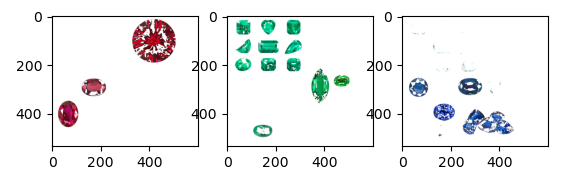
\includegraphics[width=.8\textwidth]{img/couleurs_isolees}
\end{center}
\vspace{-0.8cm}
\caption{\label{fig06} Images générées à partir de la photo de la figure \ref{fig05}}
\end{figure}

Pour mesurer cette proximité, nous allons considérer un pixel comme un vecteur de coordonnées (R,G,B,A) (R: teneur en rouge [0..1], G: teneur en vert [0..1], B: teneur en bleu [0..1], A: opacité [0..1]). 

Deux pixels A et B seront considérés proches si la norme de leur différence est inférieure à un seuil $s$.

\begin{center}
 $\sqrt{(R_A-R_B)^2+(G_A-G_B)^2+(B_A-B_B)^2+(A_A-A_B)^2}<s$
\end{center}

\question{\textbf{Écrire} une fonction \verb?norme(vec)? qui prend en entrée un vecteur, sous la forme d'une liste de dimension $n$, et retourne sa norme quel que soit $n$. Montrer que \verb?norme([1,2,3])? renvoie \verb?3.7416573867739413?.}

\question{\textbf{Recopier} et \textbf{compléter} le code suivant afin que tous les pixels pour lesquels la norme est supérieure au seuil soit coloriés en blanc.}

\newpage

\begin{minted}{python}
import copy

seuil=0.8
red,green,blue=[1,0,0,1],[0,1,0,1],[0,0,1,1]
img_coul=[]

for i in range(3):
    img_coul.append(image_couleurs.copy())
for idx,couleur in enumerate([red,green,blue]):
    for i in range(taille[0]):
        for j in range(taille[1]):
                if norme(img_coul[idx][i,j]-couleur)>seuil:
                    ..............................
f, axarr = plt.subplots(1,3)
for i in range(3):
    axarr[i].imshow(img_coul[i])
plt.show()
\end{minted}

\subsection{Compter les bijoux}

Afin de compter le nombre de bijoux, nous allons dans cette partie \textbf{détecter} les contours des bijoux puis \textbf{parcourir} l'image à l'aide d'un parcours de graphe. Cette dernière étape qui n'est pas demandée permettra de compter le nombre de cycles dans la figure et d'en déduire le nombre de bijoux.

Afin de détecter les contours sur la figure, nous allons dans un premier temps convertir la figure en noir et blanc.

\question{\textbf{Coder} la fonction \texttt{convert\_nb(image)} qui convertit une image (en couleur) en niveaux de gris.}

\question{\textbf{Coder} la fonction \texttt{contour(image\_nb)} qui convertit une image (en niveaux de gris) en contours.}

\question{\textbf{Afficher} les images obtenues à l'aide du code suivant.}

\begin{minted}{python}
f, axarr = plt.subplots(1,3)
axarr[0].imshow(image_couleurs)
axarr[0].title.set_text('Image originale')
axarr[1].imshow(image_nb)
axarr[1].title.set_text('NB')
axarr[2].imshow(contours)
axarr[2].title.set_text('Contour')
plt.show()
\end{minted}

\question{\textbf{Donner} les limites de la méthode utilisée, quelle autre approche aurait pu être utilisée pour ce cas de figure ?}

\begin{center}
\Large{FIN}
\end{center}

\end{document}}{\cleardoublepage\pagestyle{correction}}


\begin{center}
\Large{Correction}
\end{center}

\reponse{}

\begin{minted}{python}
import matplotlib.image as img
import matplotlib.pyplot as plt

parchemin1 = img.imread('parchemin1.png')
parchemin2 = img.imread('parchemin2.png')
parchemin3 = img.imread('parchemin3.png')

print(parchemin1)
plt.imshow(parchemin1)
plt.show()
\end{minted}

\reponse{}

\begin{minted}{python}
import numpy as np

parchemin=parchemin1+parchemin2+parchemin3

taille=np.shape(parchemin)

for i in range(taille[0]):
    for j in range(taille[1]):
        for k in range(taille[2]):
            if parchemin[i,j,k]>1:
                parchemin[i,j,k]=1

plt.imshow(parchemin)
plt.show()
\end{minted}

\reponse{}

\begin{minted}{python}
def dmstodd(coord,dir):
    if dir=='W' or dir=='S':
        signe=-1
    else:
        signe=1
    return signe*(coord[0]+coord[1]/60+coord[2]/3600)
    
print(dmstodd([20,37,42],'N'))
#20 37 42N
y=dmstodd([20,37,42],'N')
\end{minted}

\reponse{}

\begin{minted}{python}
#70 52 15W
x1=dmstodd([70,52,15],'W')

#enlever 2°20'13,82"
x2=dmstodd([70-2,52-20,15-13.82],'W')

def distance(stationA,stationB):
    rayon_terre=6361
    phi1=stationA[0]*np.pi/180
    phi2=stationB[0]*np.pi/180
    deltalambda=(stationB[1]-stationA[1])*np.pi/180
    return np.arccos(np.sin(phi1)*np.sin(phi2)+np.cos(phi1)*np.cos(phi2)*np.cos(deltalambda))*rayon_terre

print("Il leur a fallu parcourir {:.2f} km.".format(distance([x1,y],[x2,y])))
\end{minted}

\reponse{}

\begin{minted}{python}
diamants = img.imread('tresor.png')
taille=np.shape(diamants)
plt.imshow(diamants)
plt.show()

image_couleurs=np.ones(taille)-diamants
image_couleurs[:,:,3]=1
plt.imshow(image_couleurs)
plt.show()

#3 rouges rubis
#8 bleus  saphirs
#12 verts emeraudes
\end{minted}

\reponse{}

\begin{minted}{python}
def norme(vec):
    s=0
    for i in range(len(vec)):
        s+=vec[i]**2
    return np.sqrt(s)
\end{minted}

\reponse{}

\begin{minted}{python}
import copy

seuil=0.8

red=[1,0,0,1]
green=[0,1,0,1]
blue=[0,0,1,1]

img_coul=[]
for i in range(3):
    img_coul.append(image_couleurs.copy())

for idx,couleur in enumerate([red,green,blue]):
    for i in range(taille[0]):
        for j in range(taille[1]):
                if norme(img_coul[idx][i,j]-couleur)>seuil:
                    img_coul[idx][i,j]=[1,1,1,1]
                    
f, axarr = plt.subplots(1,3)
for i in range(3):
    axarr[i].imshow(img_coul[i])
plt.show()
\end{minted}

\reponse{}

\begin{minted}{python}
def convert_nb(image):
    image_out=np.zeros(np.shape(image))
    image_out[:,:,3]=1
    coefficients=[0.2125,0.7154,0.0721]
	# ou coefficients=[1/3,1/3,1/3]    
    for j in range(3):
        for i in range(3):
            image_out[:,:,j]+=image[:,:,i]*coefficients[i]
    return image_out

image_nb=convert_nb(image_couleurs)
plt.imshow(image_nb)
plt.show()
\end{minted}

\reponse{}

\begin{minted}{python}
def contour(image_nb):
    normel=[]
    nb_lig,nb_col,nb_coul=image_nb.shape
    image_out=np.zeros((nb_lig,nb_col,nb_coul))
    for i in range(2,nb_lig-2):
        for j in range(2,nb_col-2):
            p1=image_nb[i-2,j,0]
            p2=image_nb[i,j-2,0]
            p3=image_nb[i+2,j,0]
            p4=image_nb[i,j+2,0]
            norme=np.sqrt((p1-p3)**2+(p2-p4)**2)/2
            normel.append(norme)
            seuil=0.1
            if norme < seuil:
                p = 1
            else:
                p = 0
            for k in range(nb_coul-1):
                image_out[i,j,k]=p
            image_out[i,j,3]=1
    return image_out

contours=contour(image_nb)
plt.imshow(contours)
plt.show()
\end{minted}

\reponse{}

\begin{minted}{python}
f, axarr = plt.subplots(1,3)
axarr[0].imshow(image_couleurs)
axarr[0].title.set_text('Image originale')
axarr[1].imshow(image_nb)
axarr[1].title.set_text('NB')
axarr[2].imshow(contours)
axarr[2].title.set_text('Contour')
plt.show()
\end{minted}

\reponse{}{L'approche par les concours ne pourra pas compter des éléments s'ils se touchent comme les saphirs bleus. Une approche par intelligence artificielle, en effectuant un apprentissage au préalable serait plus judicieuse et plus efficace.}


\end{document}
